\documentclass{beamer}

%\usetheme{Madrid}
%\setbeamercovered{dynamic}
\usepackage{sansmathaccent}
\usepackage{subcaption}
\usepackage{xcolor,mathptmx,tikz,mathtools,booktabs}
\usepackage{amsmath,amssymb}
\usetikzlibrary{arrows,positioning}
\pdfmapfile{+sansmathaccent.map}

\graphicspath{{../TFM/figures/}}

\newcommand{\R}{\mathbb{R}}
\newcommand{\E}{\mathbb{E}}
\newcommand{\Q}{\mathbb{Q}}
\newcommand{\F}{\mathcal{F}}
\newcommand{\ivol}{\sigma_{\mathrm{iv}}}   % implied (Black-Scholes) volatility
\newcommand{\lvol}{\sigma_{\mathrm{loc}}}  % local (Dupire) volatility

\title{Calibration of Local Volatility Models}
\subtitle{A Tikhonov regularization approach to the Dupire inverse problem}
\author{Marc Jovani Bertran}
\date{ }
\institute{
 \small
 Tutor: Prof. Miguel Sama \\[6pt]

 Facultad de Ciencias

 Universidad Nacional de Educaci\'{o}n a Distancia (UNED) \\[6pt]

 M\'aster Universitario en Matem\'aticas Avanzadas \\
 Especialidad Matem\'aticas Aplicadas \\[6pt]

 
\includegraphics[width=1.6cm]{uned-logo.jpg}
}

\begin{document}
\frame{\titlepage}

% ----------------------------------
%   Introduction and structure of the work
% ----------------------------------

\begin{frame}
\frametitle{Introduction}
\begin{scriptsize}
\begin{itemize}
\item An option gives its holder the right, but not the obligation,
to buy (call) or sell (put) an asset at an agreed price $K$ on an agreed date $T$.

\item In 1973 Black, Scholes and Merton priced European options with a PDE
whose solution has a closed form, assuming a \textbf{constant volatility} $\sigma$.

\item After the 1987 crash markets display the \textbf{smile}:
the volatility implied by the prices depends on the strike and the maturity.

\item Dupire (1994) proposed the \textbf{local volatility model},
where the volatility is a deterministic function $\lvol(t,S)$,
which reproduces any arbitrage-free set of prices.

\item To be useful the model must be \textbf{calibrated}:
find the coefficient $\lvol$ of a PDE from finitely many, noisy observations of its solution.
This is an ill-posed \textbf{inverse problem}.
\end{itemize}
\medskip

\textbf{Aim}: build the pricing theory up to the Dupire equation,
and solve its calibration by Tikhonov regularization following

\smallskip
Egger, H., Engl, H. W. (2005). \emph{Tikhonov regularization applied to the inverse problem of option pricing: convergence analysis and rates}. Inverse Problems, 21(3), 1027.

\smallskip
All the code can be found in \url{https://github.com/M315/TFM}.
\end{scriptsize}
\end{frame}

\begin{frame}
\frametitle{Structure of the work}
\begin{scriptsize}
\begin{enumerate}
\item[2--3.] \textbf{Preliminaries.} Probability spaces, filtrations, martingales, Brownian motion,
It\^{o} integral, It\^{o} formula and SDEs.
\item[4.] \textbf{Black-Scholes.} Replication, the BS PDE, its solution, implied volatility and its surface.
\item[5.] \textbf{Arbitrage theory.} PDE and martingale methods, fundamental theorems of asset pricing.
\item[6.] \textbf{Local volatility.} Dupire formula, forward equation, no-arbitrage conditions,
local vs.\ implied volatility.
\item[7.] \textbf{Calibration.} Ill-posedness, Tikhonov functional, adjoint gradient,
convergence rates, discretization and numerical experiments.
\item[A--C.] \textbf{Appendices.} Implied volatility pipeline, calibration details, code.
\end{enumerate}
\end{scriptsize}

\begin{center}
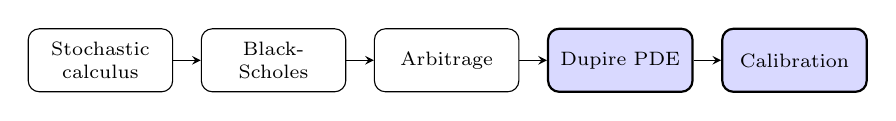
\begin{tikzpicture}[
    node distance=0.35cm,
    box/.style={draw, rounded corners, align=center, font=\scriptsize, minimum height=0.8cm, text width=1.6cm},
    focus/.style={box, fill=blue!15, thick},
    every path/.style={->, >=stealth}]
    \node[box] (sc) {Stochastic calculus};
    \node[box, right=of sc] (bs) {Black-Scholes};
    \node[box, right=of bs] (arb) {Arbitrage};
    \node[focus, right=of arb] (dup) {Dupire PDE};
    \node[focus, right=of dup] (cal) {Calibration};
    \draw (sc) -- (bs); \draw (bs) -- (arb); \draw (arb) -- (dup); \draw (dup) -- (cal);
\end{tikzpicture}
\end{center}
\begin{scriptsize}
This presentation briefly recalls stochastic calculus and Black-Scholes, and focuses on the Dupire PDE and its calibration.
\end{scriptsize}
\end{frame}

% ----------------------------------
%   Stochastic calculus (Chapter 3)
% ----------------------------------

\begin{frame}
\frametitle{Stochastic calculus. It\^{o} integral and It\^{o}'s formula}
\begin{scriptsize}
\begin{itemize}
\item An ODE $dS_t = f(t, S_t)\, dt$ cannot capture the random fluctuations of prices.
A \textbf{stochastic differential equation} adds a Brownian noise term,
\begin{equation*}
    dS_t = b(t, S_t)\, dt + \sigma(t, S_t)\, dW_t
    \iff
    S_t = S_0 + \int_0^t b(s, S_s)\, ds + \int_0^t \sigma(s, S_s)\, dW_s .
\end{equation*}
\item \textbf{It\^{o} integral}: for elementary $\phi = \sum_j e_j \mathbf{1}_{[t_j, t_{j+1})}$, with $e_j$ $\F_{t_j}$-measurable,
\begin{equation*}
    \int_0^T \phi\, dW_t = \sum_j e_j \bigl( W_{t_{j+1}} - W_{t_j} \bigr),
    \qquad
    \E\Bigl[ \Bigl( \int_0^T \phi\, dW_t \Bigr)^2 \Bigr] = \E\Bigl[ \int_0^T \phi^2\, dt \Bigr],
\end{equation*}
the second identity being the \textbf{It\^{o} isometry}. It is
extended by density to adapted processes with $\E \int_0^T f^2\, dt < \infty$.
The result is a continuous \textbf{martingale}.
\item \textbf{It\^{o}'s formula} (stochastic chain rule): if $dX_t = \mu\, dt + \sigma\, dW_t$
and $g \in C^{1,2}$, then $Y_t = g(t, X_t)$ is an It\^{o} process with
\begin{equation*}
    dY_t = \frac{\partial g}{\partial t}\, dt
        + \frac{\partial g}{\partial x}\, dX_t
        + \frac{1}{2} \frac{\partial^2 g}{\partial x^2} (dX_t)^2,
    \qquad
    (dW_t)^2 = dt,\ \ dt\, dW_t = (dt)^2 = 0 .
\end{equation*}
\item The extra second-order term $\tfrac{1}{2} \sigma^2 g_{xx}\, dt$ is what turns
stochastic dynamics into the \textbf{diffusion term of a PDE}.
\end{itemize}
\smallskip
{\O}ksendal, B. (2010). \emph{Stochastic Differential Equations}. Springer. Ch.~3--4.
\end{scriptsize}
\end{frame}

\begin{frame}
\frametitle{Stochastic calculus. SDEs as building blocks}
\begin{scriptsize}
\begin{itemize}
\item \textbf{Existence and uniqueness}: if $b$ and $\sigma$ are Lipschitz in $x$ and have linear growth,
the SDE has a unique continuous adapted solution.
\item \textbf{Geometric Brownian motion}. Applying It\^{o}'s formula to $\ln S_t$,
\begin{equation*}
    dS_t = \mu S_t\, dt + \sigma S_t\, dW_t
    \ \Longrightarrow\
    d(\ln S_t) = \Bigl( \mu - \frac{\sigma^2}{2} \Bigr) dt + \sigma\, dW_t,
\end{equation*}
so $S_t = S_0 \exp\bigl[ (\mu - \sigma^2/2) t + \sigma W_t \bigr]$. Log-normal prices, always positive: the Black-Scholes model.
\item Each model of this work is an SDE for the underlying, differing only in the diffusion coefficient:
\end{itemize}
\end{scriptsize}

\begin{center}
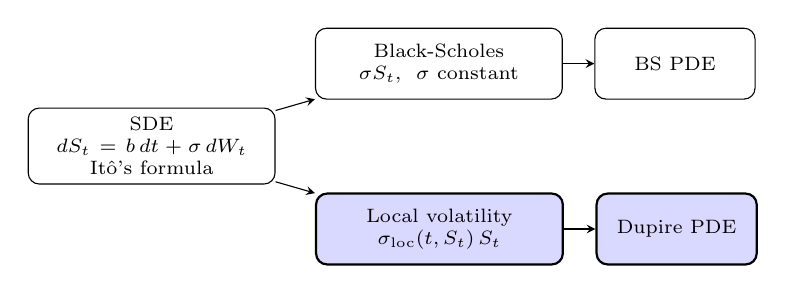
\begin{tikzpicture}[
    node distance=0.5cm and 0.6cm,
    box/.style={draw, rounded corners, align=center, font=\scriptsize, minimum height=0.9cm, text width=2.9cm},
    focus/.style={box, fill=blue!15, thick},
    every path/.style={->, >=stealth}]
    \node[box] (sde) {SDE \\ $dS_t = b\, dt + \sigma\, dW_t$ \\ It\^{o}'s formula};
    \node[box, above right=0.1cm and 0.5cm of sde] (bs) {Black-Scholes \\ $\sigma S_t$, \ $\sigma$ constant};
    \node[focus, below right=0.1cm and 0.5cm of sde] (lv) {Local volatility \\ $\lvol(t, S_t)\, S_t$};
    \node[box, right=0.4cm of bs, text width=1.8cm] (bspde) {BS PDE};
    \node[focus, right=0.4cm of lv, text width=1.8cm] (dpde) {Dupire PDE};
    \draw (sde) -- (bs); \draw (sde) -- (lv);
    \draw (bs) -- (bspde); \draw (lv) -- (dpde);
\end{tikzpicture}
\end{center}

\begin{scriptsize}
{\O}ksendal, B. (2010). \emph{Stochastic Differential Equations}. Springer. Thm.~5.2.1.
\end{scriptsize}
\end{frame}

% ----------------------------------
%   Black-Scholes (Chapter 4)
% ----------------------------------

\begin{frame}
\frametitle{Black-Scholes. Dynamic replication}
\begin{scriptsize}
\begin{itemize}
\item Arbitrage-free market, constant rate $r$, continuous rebalancing.
The underlying and the bond follow
\begin{equation*}
    dS_t = \mu S_t\, dt + \sigma S_t\, dW_t,
    \qquad
    d\beta_t = r \beta_t\, dt.
\end{equation*}
\item Replicating portfolio $V_t = a_t S_t + b_t \beta_t$ with $V_T = (S_T - K)^+$,
and \textbf{self-financing}
\begin{equation*}
    dV_t = a_t\, dS_t + b_t\, d\beta_t .
\end{equation*}
\item Writing $V_t = f(t, S_t)$, applying It\^{o}'s formula and matching the $dW_t$ and $dt$ terms,
\begin{equation*}
    a_t = \frac{\partial f}{\partial S} \quad \text{(delta hedge)},
\end{equation*}
which gives the \textbf{Black-Scholes PDE}
\begin{equation*}
    \frac{\partial f}{\partial t} =
        r f
        - r S \frac{\partial f}{\partial S}
        - \frac{1}{2} \sigma^2 S^2 \frac{\partial^2 f}{\partial S^2},
    \qquad f(T, S) = (S - K)^+ .
\end{equation*}
\item The drift $\mu$ does not appear: the price does not depend on the investors' view of the asset.
\end{itemize}
\smallskip
Black, F., Scholes, M. (1973). \emph{The Pricing of Options and Corporate Liabilities}. J. Political Economy.\\
Steele, J. M. (2010). \emph{Stochastic Calculus and Financial Applications}. Springer.
\end{scriptsize}
\end{frame}

\begin{frame}
\frametitle{Black-Scholes. Pricing formula}
\begin{scriptsize}
\begin{itemize}
\item With $\tau = T - t$, log-moneyness $x = \ln(S/K)$ and $u = e^{\alpha x + \beta \tau} v$
for suitable $\alpha, \beta$, the BS PDE reduces to the \textbf{heat equation}
\begin{equation*}
    v_\tau = \tfrac{1}{2} \sigma^2 v_{xx},
    \qquad v(x, 0) = K e^{-\alpha x} (e^x - 1)^+ .
\end{equation*}
\item Convolving with the heat kernel and completing the square gives the \textbf{Black-Scholes formula}
\begin{equation*}
    f(t, S) = S\, \Phi(d_1) - K e^{-r (T - t)} \Phi(d_2),
\end{equation*}
\begin{equation*}
    d_{1,2} = \frac{\ln(S/K) + \left( r \pm \frac{1}{2} \sigma^2 \right) (T - t)}{\sigma \sqrt{T - t}} .
\end{equation*}
\item \textbf{Implied volatility}: the unique $\ivol(K,T) > 0$ such that
$C_{\mathrm{BS}}(\ivol) = C^{\mathrm{mkt}}$.
Uniqueness follows from the vega
\begin{equation*}
    \mathcal{V} = \frac{\partial C_{\mathrm{BS}}}{\partial \sigma} = S \sqrt{T - t}\, \phi(d_1) > 0,
\end{equation*}
and it is computed with Newton's method
$\sigma^{(n+1)} = \sigma^{(n)} - \bigl(C_{\mathrm{BS}}(\sigma^{(n)}) - C^{\mathrm{mkt}}\bigr) / \mathcal{V}(\sigma^{(n)})$.
\end{itemize}
\end{scriptsize}
\end{frame}

\begin{frame}
\frametitle{Black-Scholes. The implied volatility surface}
\begin{scriptsize}
If Black-Scholes described the market, $\ivol(K,T)$ would be flat.
SPY quotes on 30 April 2026 show a \textbf{negative skew} in strike and a \textbf{term structure} in maturity.
\end{scriptsize}
\begin{figure}[htb!]
    \centering
    \begin{subfigure}[b]{0.55\linewidth}\centering
    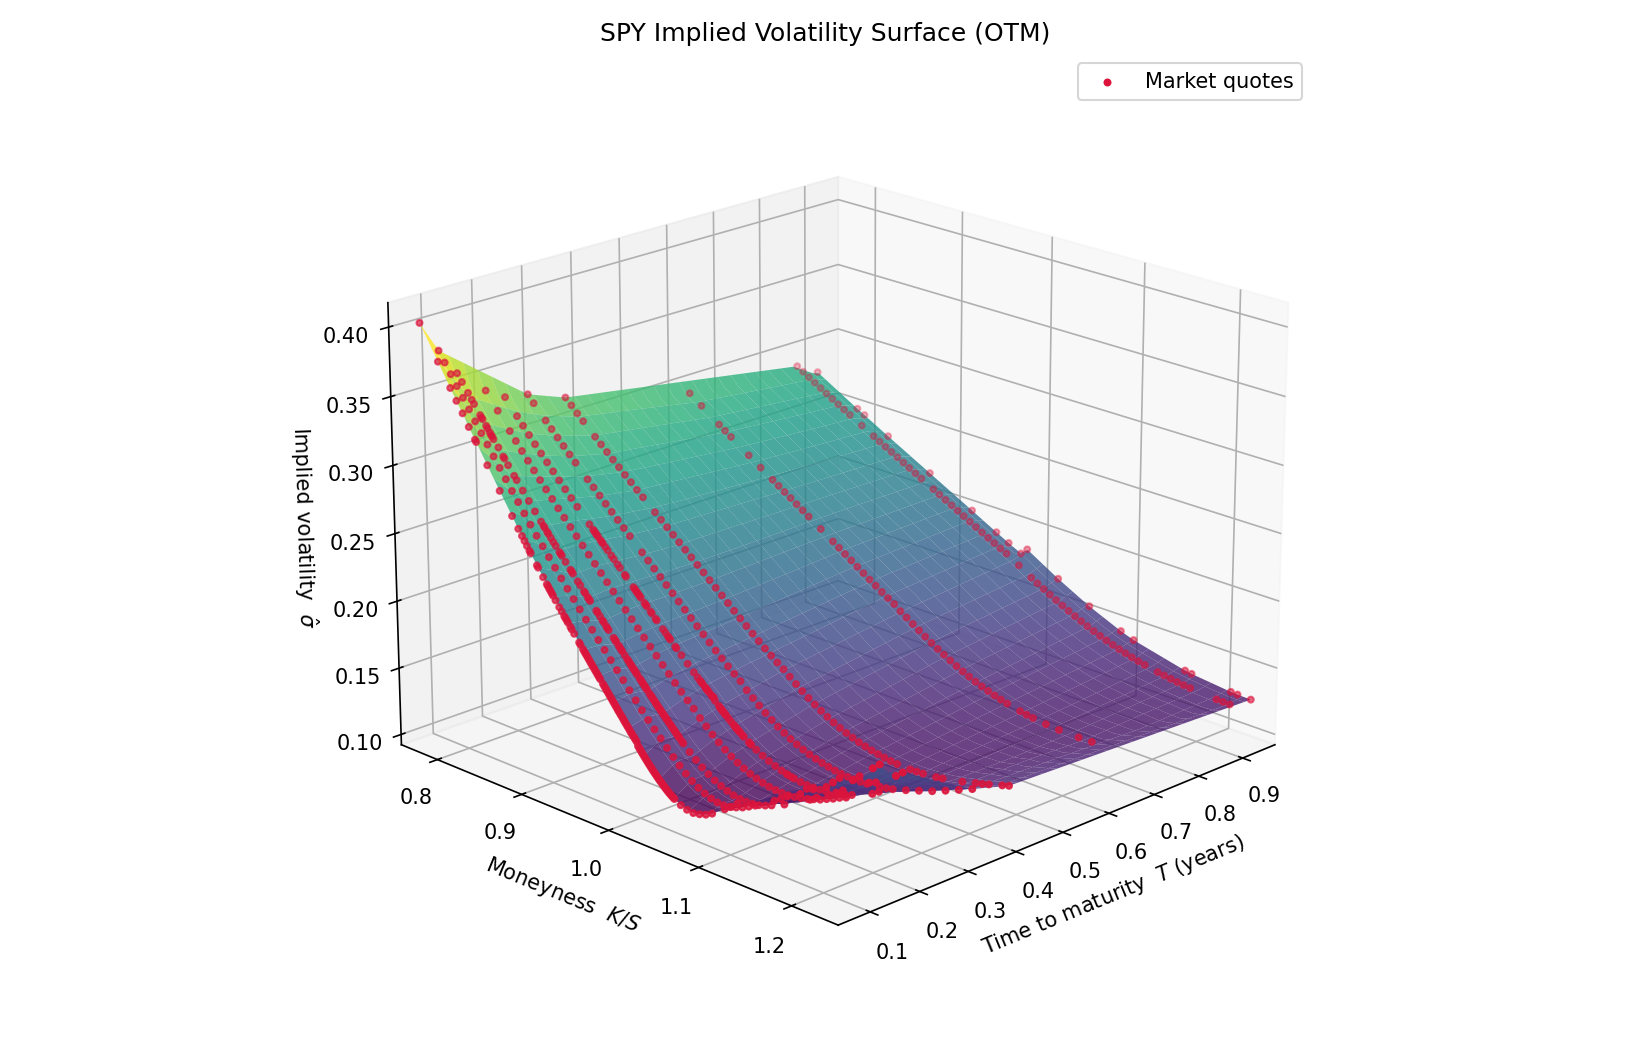
\includegraphics[width=\linewidth]{iv_composite}
    \caption{\scriptsize Implied volatility surface.}
    \end{subfigure}%
    \begin{subfigure}[b]{0.45\linewidth}\centering
    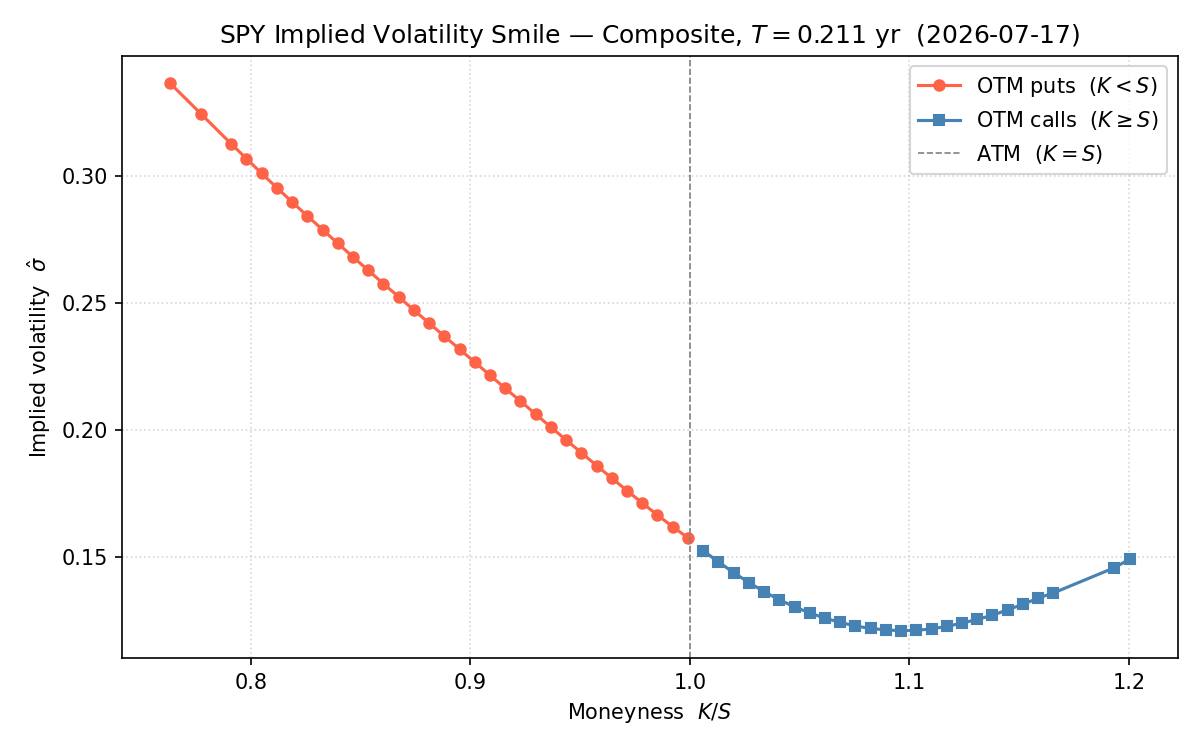
\includegraphics[width=\linewidth]{iv_smile}
    \caption{\scriptsize Smile at $T \approx 0.21$.}
    \end{subfigure}
\end{figure}
\begin{scriptsize}
Constant $\sigma$ is inconsistent with the market, which motivates the local volatility model.
\end{scriptsize}
\end{frame}

% ----------------------------------
%   Arbitrage theory (Chapter 5)
% ----------------------------------

\begin{frame}
\frametitle{Arbitrage theory. Market, portfolios and arbitrage}
\begin{scriptsize}
\begin{itemize}
\item \textbf{Market}: a riskless asset $dS_0 = r S_0\, dt$ and risky assets
\begin{equation*}
    dS_i(t) = \mu_i(S(t), t)\, dt + \sigma_i(S(t), t)^\intercal dW(t), \qquad i = 1, \dots, n .
\end{equation*}
\item \textbf{Portfolio}: an adapted process $\theta(t)$ with value $V(t) = \theta(t)^\intercal S(t)$,
self-financing if $dV(t) = \theta(t)^\intercal dS(t)$.

\item \textbf{PDE method}: replicating $V(S(t), t)$ and imposing self-financing gives
$\theta_i = \partial V / \partial S_i$ and
\begin{equation*}
    \frac{\partial V}{\partial t} + \frac{1}{2} \sum_{i,j} \frac{\partial^2 V}{\partial S_i \partial S_j} \sigma_i^\intercal \sigma_j = 0,
    \qquad V = \sum_{i} \frac{\partial V}{\partial S_i} S_i,
\end{equation*}
which recovers the BS PDE for $n = 1$, $\sigma_1 = \sigma S_1$.

\item \textbf{Arbitrage}: a self-financing admissible portfolio with
\begin{enumerate}
\item $V(0) < 0$ and $\mathbb{P}(V(t) \geq 0) = 1$, or
\item $V(0) = 0$, $\mathbb{P}(V(t) \geq 0) = 1$ and $\mathbb{P}(V(t) > 0) > 0$.
\end{enumerate}
\end{itemize}
\smallskip
Bj\"ork, T. (2009). \emph{Arbitrage Theory in Continuous Time}. Oxford University Press.\\
Glasserman, P. (2003). \emph{Monte Carlo Methods in Financial Engineering}. Springer.
\end{scriptsize}
\end{frame}

\begin{frame}
\frametitle{Arbitrage theory. Martingale method}
\begin{scriptsize}
\begin{itemize}
\item A \textbf{risk-neutral measure} $\Q \sim \mathbb{P}$ is one under which the normalized prices
$Z_i = S_i / S_0$ are martingales: every asset drifts at the risk-free rate.

\item \textbf{First fundamental theorem.}
The market is arbitrage-free if and only if there exists an equivalent (local) martingale measure $\Q$.

\item \textbf{Second fundamental theorem.}
Assuming no arbitrage, the market is complete if and only if $\Q$ is unique.

\item In a complete market the price of a claim with payoff $f(S(T))$ is
\begin{equation*}
    V(t) = \E^{\Q} \left[ \left. e^{ - \int^T_t r(s)\, ds} f(S(T)) \,\right| \F_t \right].
\end{equation*}
\end{itemize}
\medskip
For a call with constant $r$,
\begin{equation*}
    C(K, T) = e^{-rT}\, \E^{\Q}\!\left[(S_T - K)^+\right],
\end{equation*}
which is the starting point of the Dupire equation.
\end{scriptsize}
\end{frame}

% ----------------------------------
%   Local volatility and the Dupire PDE (Chapter 6)
% ----------------------------------

\begin{frame}
\frametitle{Local volatility model}
\begin{scriptsize}
\begin{itemize}
\item The volatility becomes a deterministic function of time and spot,
\begin{equation*}
    \frac{dS_t}{S_t} = (r - q)\, dt + \lvol(t, S_t)\, dW_t ,
\end{equation*}
with $q$ the dividend yield.
We write $\lvol$ for the local and $\ivol$ for the implied volatility.

\item The pricing PDE is the Black-Scholes one with $\sigma$ replaced by $\lvol(t,S)$,
\begin{equation*}
    \frac{\partial f}{\partial t} =
        r f
        - (r - q) S \frac{\partial f}{\partial S}
        - \frac{1}{2} \lvol^2(t, S) S^2 \frac{\partial^2 f}{\partial S^2}.
\end{equation*}

\item It is a \textbf{market model}: it is calibrated so that vanilla options are priced exactly.

\item \textbf{Question}: given the call prices $C(K,T)$, which $\lvol$ produces them?
\end{itemize}
\medskip
Dupire, B. (1994). \emph{Pricing with a Smile}. Risk.\\
Bergomi, L. (2015). \emph{Stochastic Volatility Modeling}, Ch.~2. CRC Press.
\end{scriptsize}
\end{frame}

\begin{frame}
\frametitle{Dupire equation. Derivation (I)}
\begin{scriptsize}
Take a general diffusion $dS_t = (r - q) S_t\, dt + \sigma_t S_t\, dW_t$, $\sigma_t$ any adapted process,
and undiscounted prices $\mathcal{C}(K,T) = e^{rT} C(K,T) = \E[(S_T - K)^+]$.
\begin{itemize}
\item In the sense of distributions, with $\theta$ the Heaviside function and $\delta$ the Dirac delta,
\begin{equation*}
    \frac{d}{dx}(x)^+ = \theta(x),
    \qquad
    \frac{d^2}{dx^2}(x)^+ = \delta(x).
\end{equation*}
\item It\^{o}'s formula applied to $(S_T - K)^+$ over $[T, T + dT]$,
\begin{equation*}
    d(S_T - K)^+
    = \theta(S_T - K)\bigl((r-q) S_T\, dT + \sigma_T S_T\, dW_T\bigr)
    + \tfrac{1}{2}\,\delta(S_T - K)\,\sigma_T^2 S_T^2\, dT.
\end{equation*}
\item Differentiating $\mathcal{C}$ in $K$,
\begin{equation*}
    \E\!\left[\theta(S_T - K)\right] = -\frac{\partial \mathcal{C}}{\partial K},
    \qquad
    \E\!\left[\delta(S_T - K)\right] = \frac{\partial^2 \mathcal{C}}{\partial K^2} = p^*(K, T),
\end{equation*}
the second one is \textbf{Breeden-Litzenberger}: the convexity in strike is the risk-neutral density of $S_T$.
\end{itemize}
\medskip
Breeden, D. T., Litzenberger, R. H. (1978). \emph{Prices of State-Contingent Claims Implicit in Option Prices}. J. Business.
\end{scriptsize}
\end{frame}

\begin{frame}
\frametitle{Dupire equation. Derivation (II)}
\begin{scriptsize}
\begin{itemize}
\item Taking expectations ($\E[dW_T] = 0$) and using the sifting property $S_T^2\,\delta(S_T - K) = K^2\,\delta(S_T - K)$,
\begin{equation*}
    \frac{\partial \mathcal{C}}{\partial T}
    = (r-q)\left(\mathcal{C} - K\frac{\partial \mathcal{C}}{\partial K}\right)
    + \frac{K^2}{2}\,\E\!\left[\sigma_T^2\,\delta(S_T - K)\right].
\end{equation*}
\item Dividing by $\E[\delta(S_T - K)]$ and going back to discounted prices,
\begin{equation*}
    \E\!\left[\sigma_T^2 \,\middle|\, S_T = K\right]
    = 2\,\frac{\dfrac{\partial C}{\partial T} + qC + (r-q)\,K\,\dfrac{\partial C}{\partial K}}
           {K^2\,\dfrac{\partial^2 C}{\partial K^2}},
\end{equation*}
valid for \emph{any} $\sigma_t$: the smile only fixes the conditional expectation of $\sigma_T^2$.

\item In the local volatility model $\sigma_t = \lvol(t, S_t)$, which gives the \textbf{Dupire formula}
\begin{equation*}
    \lvol(t, S)^2 = 2\,\frac{
        \dfrac{\partial C}{\partial T} + qC + (r-q)\,K\,\dfrac{\partial C}{\partial K}
    }{
        K^2\,\dfrac{\partial^2 C}{\partial K^2}
    }\Bigg|_{\substack{K = S,\\ T = t}}.
\end{equation*}
\item A full surface of call prices determines $\lvol$ uniquely.
\end{itemize}
\end{scriptsize}
\end{frame}

\begin{frame}
\frametitle{Dupire forward equation}
\begin{scriptsize}
Rearranging the same identity, for a known $\lvol$ the call prices solve the \textbf{Dupire forward equation}
\begin{equation}\label{eq:dupire_forward}
    \frac{\partial C}{\partial T} + (r-q)\,K\,\frac{\partial C}{\partial K}
    - \frac{\lvol^2(T,K)}{2}\,K^2\,\frac{\partial^2 C}{\partial K^2} = -qC,
\end{equation}
\begin{equation*}
    (K, T) \in (0, \infty) \times (0, T_{\max}], \qquad C(K, 0) = (S_0 - K)^+ .
\end{equation*}

\begin{center}
\begin{tabular}{l l l}
\toprule
 & Black-Scholes PDE & Dupire PDE \\
\midrule
Variables & spot $S$, time $t$ & strike $K$, maturity $T$ \\
Direction & backward from payoff at $T$ & forward from $T = 0$ \\
Fixed & one strike and maturity & one spot $S_0$ \\
Output & price for every $S$ & prices for every $(K, T)$ \\
\bottomrule
\end{tabular}
\end{center}
\medskip

\begin{itemize}
\item One solve prices the whole surface quoted today.
This is what makes the equation the natural \textbf{direct problem} for calibration:
the data $C^*(K_i, T_j)$ are values of its solution, and the unknown is its coefficient $\lvol$.
\end{itemize}
\end{scriptsize}
\end{frame}

\begin{frame}
\frametitle{No-arbitrage conditions}
\begin{scriptsize}
No arbitrage makes numerator and denominator of the Dupire formula non-negative,
so $\lvol^2 \geq 0$ wherever the density of $S_T$ does not vanish.
\begin{itemize}
\item \textbf{Strike (butterfly) arbitrage.}
$\partial^2 C / \partial K^2 = e^{-rT} p^*(K,T) \geq 0$.
Otherwise the butterfly
\begin{equation*}
    V_0(\varepsilon)
        = \frac{C(K-\varepsilon, T) - 2\,C(K, T) + C(K+\varepsilon, T)}{\varepsilon^2}
        \longrightarrow \frac{\partial^2 C}{\partial K^2} < 0
\end{equation*}
is entered at a negative premium with a non-negative payoff, by convexity of $(x)^+$.

\item \textbf{Maturity (calendar) arbitrage.}
The numerator equals
\begin{equation*}
    e^{-qT}\frac{d}{dT}\!\left[e^{qT}\,C\!\left(K e^{(r-q)T}, T\right)\right] \geq 0,
\end{equation*}
a call struck at a fixed proportion of the forward cannot get cheaper with maturity.
\end{itemize}
\medskip
Both are conditions on the \emph{prices}: every arbitrage-free surface admits a local volatility.
\end{scriptsize}
\end{frame}

\begin{frame}
\frametitle{From local to implied volatility}
\begin{scriptsize}
\begin{itemize}
\item \textbf{Gamma average.} Delta hedging with $\ivol$ while the spot follows $\lvol$ gives
\begin{equation*}
    \ivol(K,T)^2
    = \frac{
        \E\!\left[\int_0^T e^{-rt} S_t^2\,
            \partial_{SS} C_{\mathrm{BS}}\,\lvol(t, S_t)^2\,dt\right]
      }{
        \E\!\left[\int_0^T e^{-rt} S_t^2\,
            \partial_{SS} C_{\mathrm{BS}}\,dt\right]
      }:
\end{equation*}
the implied variance is a smoothed local variance, so the smile is flatter.

\item \textbf{Rule of two.} If $\lvol(t, S) = \sigma_0 + \alpha(t)\, x + \cdots$, $x = \ln(S / F_t)$,
the ATMF skew $\mathcal{S}_T = \partial_{\ln K} \ivol |_{K = F_T}$ is, to first order,
\begin{equation*}
    \mathcal{S}_T = \frac{1}{T}\int_0^T \frac{t}{T}\,\alpha(t)\,dt
    \quad \overset{\alpha \text{ const.}}{\Longrightarrow} \quad
    \mathcal{S}_T = \frac{\alpha}{2}.
\end{equation*}
The local skew is twice the implied skew.

\item \textbf{Skew stickiness ratio.}
$\mathcal{R}_T = \frac{1}{\mathcal{S}_T}\frac{d\sigma_{\mathrm{ATMF}}}{d\ln S_0} = 1 + \frac{1}{T}\int_0^T \frac{\mathcal{S}_t}{\mathcal{S}_T}\,dt$,
equal to $2$ for a flat term structure of skew:
the smile dynamics are not free, they are fixed by the calibrated smile.
\end{itemize}
\medskip
Bergomi, L. (2015). \emph{Stochastic Volatility Modeling}, Ch.~2. CRC Press.\\
Derman, E., Miller, M. B., Park, D. (2016). \emph{The Volatility Smile}. Wiley.
\end{scriptsize}
\end{frame}

% ----------------------------------
%   Calibration as an inverse problem (Chapter 7, theory)
% ----------------------------------

\begin{frame}
\frametitle{Calibration. An ill-posed inverse problem}
\begin{scriptsize}
\textbf{Data}: quoted calls $C^*(K_i, T_j)$ on finitely many strikes and maturities.
\textbf{Unknown}: the coefficient $\lvol$ of the forward equation \eqref{eq:dupire_forward}.
\medskip

Why not plug the quotes into the Dupire formula?
\begin{itemize}
\item The data are \textbf{noisy} and \textbf{sparse}, especially in maturity,
and the formula needs $\partial_T C$ and $\partial_{KK} C$.
\item Gamma $\partial_{KK} C$ sits in the denominator:
far from the money it is small and $\lvol$ is barely determined by the prices.
\item The map from $\lvol$ to prices is \textbf{smoothing}:
very different volatilities produce almost the same prices,
so its inverse is discontinuous and amplifies the noise.
\end{itemize}
\medskip
We follow Egger and Engl and stabilize the inversion by \textbf{Tikhonov regularization}.
\medskip

Egger, H., Engl, H. W. (2005). \emph{Tikhonov regularization applied to the inverse problem of option pricing: convergence analysis and rates}. Inverse Problems.\\
Engl, H. W., Hanke, M., Neubauer, A. (1996). \emph{Regularization of Inverse Problems}. Kluwer.
\end{scriptsize}
\end{frame}

\begin{frame}
\frametitle{Calibration. Log-moneyness formulation}
\begin{scriptsize}
With $y = \log(K/S_0)$, $\tau = T$, $u(y, \tau) = C/S_0$ and the diffusion coefficient
\begin{equation*}
    a(y,\tau) = \tfrac{1}{2}\lvol^2(T,K),
\end{equation*}
the operators $K\partial_K$ and $K^2\partial_{KK}$ have constant coefficients,
\begin{equation*}
    K\,\frac{\partial C}{\partial K} = S_0\,u_y,
    \qquad
    K^2\,\frac{\partial^2 C}{\partial K^2} = S_0\,(u_{yy} - u_y),
\end{equation*}
and the forward equation becomes, on $Q = (-M, M) \times (0, T]$,
\begin{equation}\label{eq:forward_y}
    u_\tau = a(y,\tau)\,(u_{yy} - u_y) - (r-q)\,u_y - q\,u,
\end{equation}
\begin{equation*}
    u(y, 0) = (1 - e^y)^+,
    \qquad u(-M, \tau) = \Psi_1(\tau), \quad u(M, \tau) = \Psi_2(\tau),
\end{equation*}
with the boundary values from Black-Scholes at $K = S_0 e^{\pm M}$
($\Psi_1 \to e^{-q\tau}$, $\Psi_2 \to 0$ as $M \to \infty$).
\end{scriptsize}
\end{frame}

\begin{frame}
\frametitle{Calibration. Parameter-to-solution map}
\begin{scriptsize}
\begin{itemize}
\item Admissible set, for a prior $a^*$ and bounds $0 < \underline{a} \leq \bar{a}$,
\begin{equation*}
    \mathcal{K}(a^*) := \bigl\{ a \in a^* + H^1(Q) : \underline{a} \le a \le \bar{a} \bigr\}.
\end{equation*}
$H^1$ is needed because $a$ enters the weak form through the flux,
and its norm gives weak compactness of the sublevel sets.

\item Parameter-to-solution map, $u(a)$ the solution of \eqref{eq:forward_y},
\begin{equation*}
    F(a) = u(a) - u(a_0), \qquad a_0 \text{ constant, } u(a_0) \text{ from Black-Scholes}.
\end{equation*}
\end{itemize}

\begin{block}{Theorem (Egger and Engl, Thm.~2.1)}
There exists $p^* > 2$ such that $F\colon \mathcal{K}(a^*) \to W_p^{2,1}(Q)$
is continuous and compact for $2 \le p < p^*$, and weakly sequentially continuous.
\end{block}

\begin{itemize}
\item This is the \textbf{source of the ill-posedness}:
a compact operator between infinite dimensional spaces has no continuous inverse,
small changes in prices may correspond to order one changes in $a$.
\end{itemize}
\end{scriptsize}
\end{frame}

\begin{frame}
\frametitle{Calibration. Tikhonov functional}
\begin{scriptsize}
Assume $a^\dagger \in \mathcal{K}(a^*)$ reproduces the true prices $u^\dagger$
and the observations satisfy $\|u^\delta - u^\dagger\|_{L^2(Q)} \le \delta$. We minimize
\begin{equation*}
    J^\beta(a) = \underbrace{\|u(a) - u^\delta\|^2_{L^2(Q)}}_{\text{data fit}}
    + \beta\,\underbrace{\|a - a^*\|^2_{H^1(\Omega)}}_{\text{smoothness, prior}},
    \qquad \Omega = (-M, M).
\end{equation*}

\begin{block}{Proposition (Egger and Engl, Props.~3.1 and 3.2)}
For any $\beta > 0$ a minimizer $a^\delta_\beta$ exists.
If $\delta \to 0$, $\beta(\delta) \to 0$ and $\delta^2/\beta(\delta) \to 0$,
the minimizers have a subsequence converging in $H^1(\Omega)$,
and every limit point is an \emph{$a^*$-minimum-norm} solution.
\end{block}

\begin{itemize}
\item The prior $a^*$ carries the structural knowledge where the data are weak.
\item With finitely many quotes the data are discrete:
convergence to an $a^*$-minimum-norm solution holds, its uniqueness does not.
\end{itemize}
\end{scriptsize}
\end{frame}

\begin{frame}
\frametitle{Calibration. Gradient by the adjoint method}
\begin{scriptsize}
\begin{itemize}
\item The directional derivative needs the linearized solution $w = u'(a)[h]$,
\begin{equation*}
    \frac{d}{d\varepsilon}\|u(a+\varepsilon h) - u^\delta\|^2\Big|_{\varepsilon=0}
    = 2\bigl(u(a) - u^\delta,\, w\bigr),
\end{equation*}
\begin{equation*}
    -w_\tau + a(w_{yy} - w_y) - (r-q) w_y - q w = -h\,(u_{yy} - u_y),
\end{equation*}
one PDE solve per direction $h$, i.e.\ $n$ solves for $n$ degrees of freedom.

\item Instead solve once the \textbf{adjoint} problem backward in $\tau$,
\begin{equation*}
    V_\tau + (aV)_{yy} + (aV)_y + (r-q)V_y - qV = 0,
    \qquad V(y, T) = u(a)(y, T) - u^\delta(y),
\end{equation*}
with homogeneous Dirichlet conditions. Then
\begin{equation*}
    \langle \nabla J^\beta(a), h \rangle
    = 2\int_0^{T}\!\!\int_{-M}^{M} h\,(u_{yy}-u_y)\,V\,dy\,d\tau
      + 2\beta\int_{-M}^{M}\bigl[(a-a^*)h + \partial_y(a-a^*)\,\partial_y h\bigr]dy.
\end{equation*}

\item Cost: \textbf{one forward and one adjoint solve per iteration},
independent of the number of unknowns.
\item $V$ represents $F'(a)^*(F(a) - u^\delta)$, the object appearing in the source condition.
\end{itemize}
\end{scriptsize}
\end{frame}

\begin{frame}
\frametitle{Calibration. Convergence rates}
\begin{scriptsize}
\begin{itemize}
\item Under the \textbf{source condition}
\begin{equation*}
    a^* - a^\dagger = F'(a^\dagger)^*\,w, \qquad \|w\| \text{ small},
\end{equation*}
and the choice $\beta \sim \delta$ (Egger and Engl, Prop.~4.1),
\begin{equation*}
    \|a^\delta_\beta - a^\dagger\| = O(\sqrt{\delta}),
    \qquad
    \|u(a^\delta_\beta) - u^\delta\| = O(\delta).
\end{equation*}

\item For time independent $a = a(y)$ and one maturity, the condition is implied by
smooth source functions $g$ with Gaussian decay in the wings
\begin{equation*}
    |g|,\ |\partial_y g|,\ |\partial_y^2 g| = O\bigl(e^{-B' y^2}\bigr), \qquad |y| \to \infty,
\end{equation*}
with an $H^2$ penalty (Thm.~4.1) or with observed digital prices $C_K$ (Thm.~4.2).

\item \textbf{Interpretation}: $a^\dagger - a^*$ must be small and smooth in the wings,
where the prices carry little information. The wings must come from the prior.
\end{itemize}
\medskip
\textbf{Caveat}: we keep the $H^1$ penalty with price data only,
and later calibrate a time dependent $a(y,\tau)$, both outside the rate theorems.
\end{scriptsize}
\end{frame}

\begin{frame}
\frametitle{Calibration. Discretization and minimization}
\begin{scriptsize}
\begin{itemize}
\item \textbf{Space}: $P_1$ Lagrange finite elements on $[-M, M]$, with FEniCSx. Weak form, $v \in H^1_0$,
\begin{equation*}
    \frac{d}{d\tau}\!\int u\,v
    = -\!\int a\,u_y\,v_y
      -\!\int \partial_y a\,u_y\,v
      -\!\int (a + r - q)\,u_y\,v
      -\!\int q\,u\,v .
\end{equation*}
\item \textbf{Time}: implicit Euler, unconditionally stable for this parabolic operator.
\item \textbf{Optimizer}: L-BFGS-B, which handles the bounds $\underline{a} \le a \le \bar a$.
\item \textbf{Choice of $\beta$}: decreasing sequence $\beta_0 = 10^{2}\delta > \cdots > 10^{-3}\delta$,
warm started, stopped by the Morozov discrepancy principle $\|u(a^\delta_\beta) - u^\delta\| \le 1.5\,\delta$.
\end{itemize}

\textbf{Gradient check.} Adjoint vs.\ linearized solve agree to $2.3\times10^{-15}$,
and the Taylor remainder $R_1(t) = |J(a+th) - J(a) - t\langle\nabla J, h\rangle|$ is $O(t^2)$:
\begin{center}
\begin{tabular}{c c c c}
\toprule
$t$ & $R_0(t)$ & $R_1(t)$ & rate of $R_1$ \\
\midrule
$10^{-2}$ & $1.32\times10^{-6}$ & $5.13\times10^{-6}$ & - \\
$10^{-3}$ & $3.28\times10^{-7}$ & $5.27\times10^{-8}$ & $1.99$ \\
$10^{-4}$ & $3.76\times10^{-8}$ & $5.29\times10^{-10}$ & $2.00$ \\
$10^{-5}$ & $3.80\times10^{-9}$ & $5.29\times10^{-12}$ & $2.00$ \\
\bottomrule
\end{tabular}
\end{center}
\end{scriptsize}
\end{frame}

% ----------------------------------
%   Calibration, numerical experiments (Chapter 7)
% ----------------------------------

\begin{frame}
\frametitle{Example 1. Constant volatility}
\begin{scriptsize}
Egger and Engl, Example 1: recover $a^\dagger = 0.15$ ($\lvol \approx 0.548$) on $y \in [-3,3]$, $\tau \in [0,1]$,
$r = q = 0$, $S_0 = 1000$, prior $a^*(y) = 0.15 - 0.05\,\operatorname{erf}(-y^2)$, $\beta = 10^{-6}$.
Cases: (A) exact data, (B) 20 strikes, (C) poor prior $a^* \equiv 0.15$, (D) $0.1\%$ noise, (BD) both.
\end{scriptsize}
\begin{center}
\begin{tiny}
\begin{tabular}{c c c c c c c}
\toprule
Strike & True & A & B & C & D & BD \\
\midrule
600  & 0.1500 & 0.1493 & 0.1500 & 0.1519 & 0.1378 & 0.1245 \\
1000 & 0.1500 & 0.1499 & 0.1499 & 0.1515 & 0.1490 & 0.1455 \\
1400 & 0.1500 & 0.1497 & 0.1498 & 0.1504 & 0.1489 & 0.1522 \\
1600 & 0.1500 & 0.1508 & 0.1501 & 0.1491 & 0.1543 & 0.1500 \\
1800 & 0.1500 & 0.1487 & 0.1504 & 0.1511 & 0.1461 & 0.1463 \\
\bottomrule
\end{tabular}
\end{tiny}
\end{center}
\begin{figure}[htb!]
    \centering
    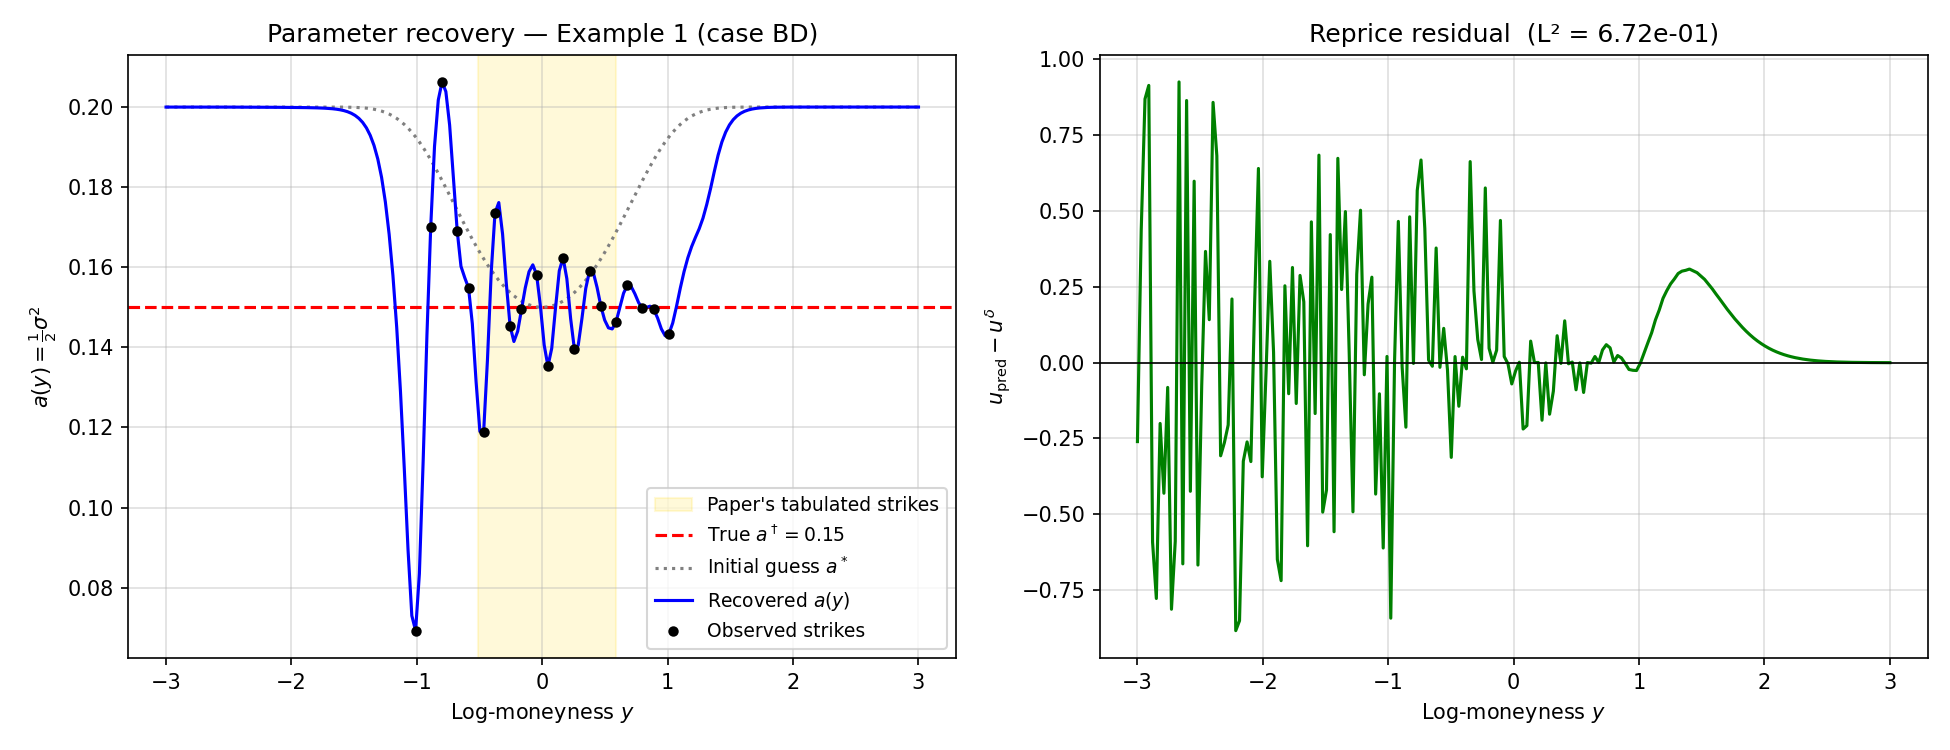
\includegraphics[width=0.8\linewidth]{egger_example1_caseBD}
    \caption{\scriptsize Case BD: incomplete and noisy data. Good recovery where observed, prior dominates the wings.}
\end{figure}
\end{frame}

\begin{frame}
\frametitle{Example 2. The role of the prior}
\begin{scriptsize}
Oscillatory true coefficient near the money,
$a^\dagger(y) = 0.15 + 0.05\,e^{-(y+0.3)^2}\sin(2\pi y) + 0.05\,\operatorname{erf}(20 y)$,
prior $a^*(y) = 0.15 + 0.05\,\operatorname{erf}(2y)$.
Data generated on a finer mesh and wider domain to avoid the \emph{inverse crime};
noisy cases use the $\beta$ schedule with the discrepancy principle.
\end{scriptsize}
\begin{figure}[htb!]
    \centering
    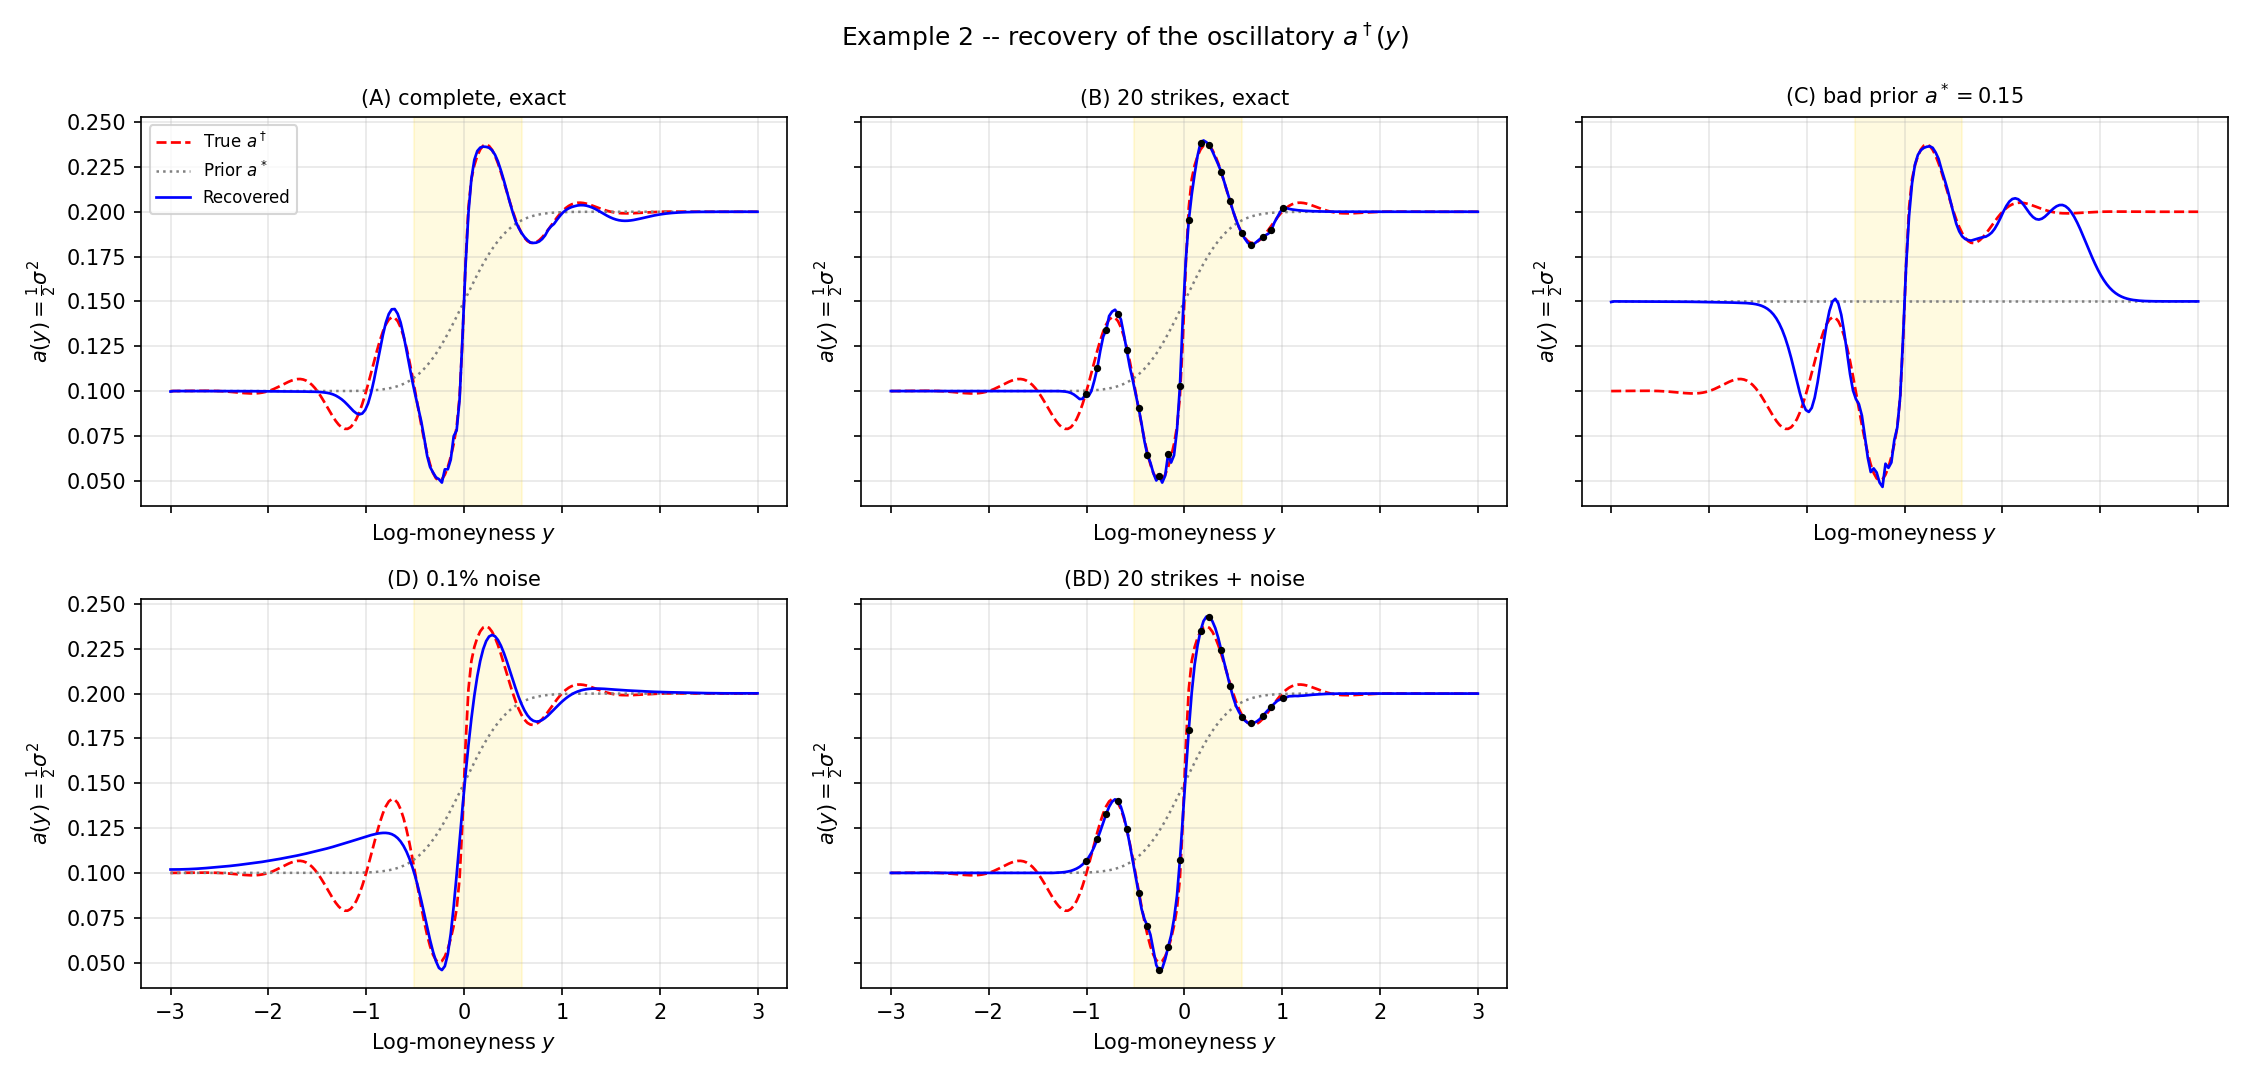
\includegraphics[width=0.9\linewidth]{egger_example2_recovery}
    \caption{\scriptsize Recovered $a(y)$ (blue), true $a^\dagger$ (red dashed), prior (grey).
    In case C the constant prior cannot recover the wings, where the data are weak.}
\end{figure}
\end{frame}

\begin{frame}
\frametitle{Market surface. Extension to time-dependent volatility}
\begin{scriptsize}
\begin{itemize}
\item Prices are observed at finitely many maturities, so $a$ is taken \textbf{piecewise constant in time},
\begin{equation*}
    a(y,\tau) = \sum_{n=1}^{K} a_n(y)\,\chi_{(\tau_{n-1},\,\tau_n]}(\tau),
    \qquad a_n \in H^1(-M,M),
\end{equation*}
one slice per quoted maturity. $K = 1$ is the setting of Egger and Engl.

\item The functional adds a penalty on jumps between slices,
\begin{equation*}
    J(a) = \sum_{j=1}^{N} \bigl\| u(a)(\cdot,\tau_j) - u^\delta_j \bigr\|^2_{L^2(\Omega_j)}
         + \beta_y \sum_{n=1}^{K} \| a_n - a^*_n \|^2_{H^1(\Omega)}
         + \beta_\tau \sum_{n=2}^{K} \| a_n - a_{n-1} \|^2_{L^2(\Omega)}.
\end{equation*}
One forward march to the last maturity and one adjoint sweep give the whole gradient.

\item \textbf{Prior.} Seeding with $\tfrac12\ivol^2$ anchors the slope at half the right value (rule of two).
Instead invert the short maturity harmonic mean relation of Berestycki, Busca and Florent,
\begin{equation*}
    \frac{y}{\ivol(y)} = \int_0^y \frac{dx}{\lvol(x)}
    \quad \Longrightarrow \quad
    \lvol(y) = \frac{\ivol(y)}{1 - y\,\partial_y\ivol(y)/\ivol(y)}.
\end{equation*}
\end{itemize}
\medskip
Berestycki, H., Busca, J., Florent, I. (2002). \emph{Asymptotics and calibration of local volatility models}. Quantitative Finance.
\end{scriptsize}
\end{frame}

\begin{frame}
\frametitle{Market surface. SPY, 30 April 2026}
\begin{scriptsize}
$S_0 = 720.65$, eleven maturities $\tau \in [0.10, 0.88]$, liquid band $0.8 \le K/S_0 \le 1.2$,
$\beta_y = 0.1$, $\beta_\tau = 1$.
\end{scriptsize}
\begin{figure}[htb!]
    \centering
    \begin{subfigure}[b]{0.5\linewidth}\centering
    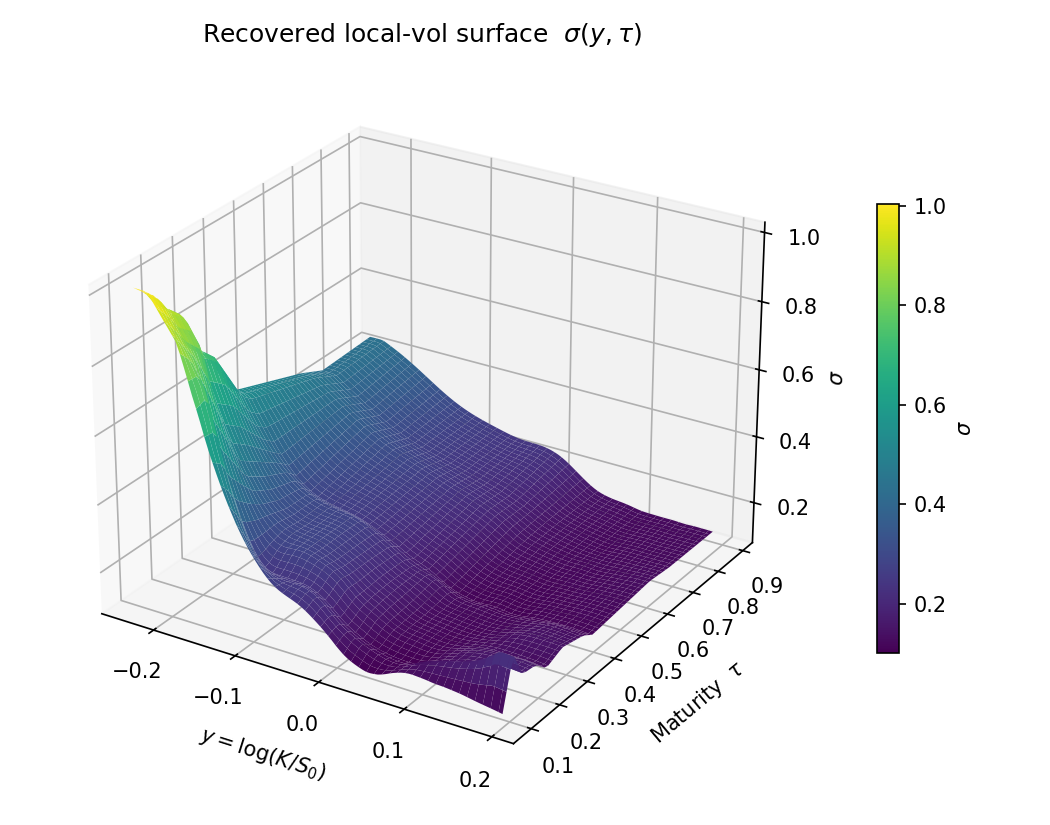
\includegraphics[width=\linewidth]{egger_example4_surface_3d}
    \caption{\scriptsize Calibrated $\lvol(y,\tau)$.}
    \end{subfigure}%
    \begin{subfigure}[b]{0.5\linewidth}\centering
    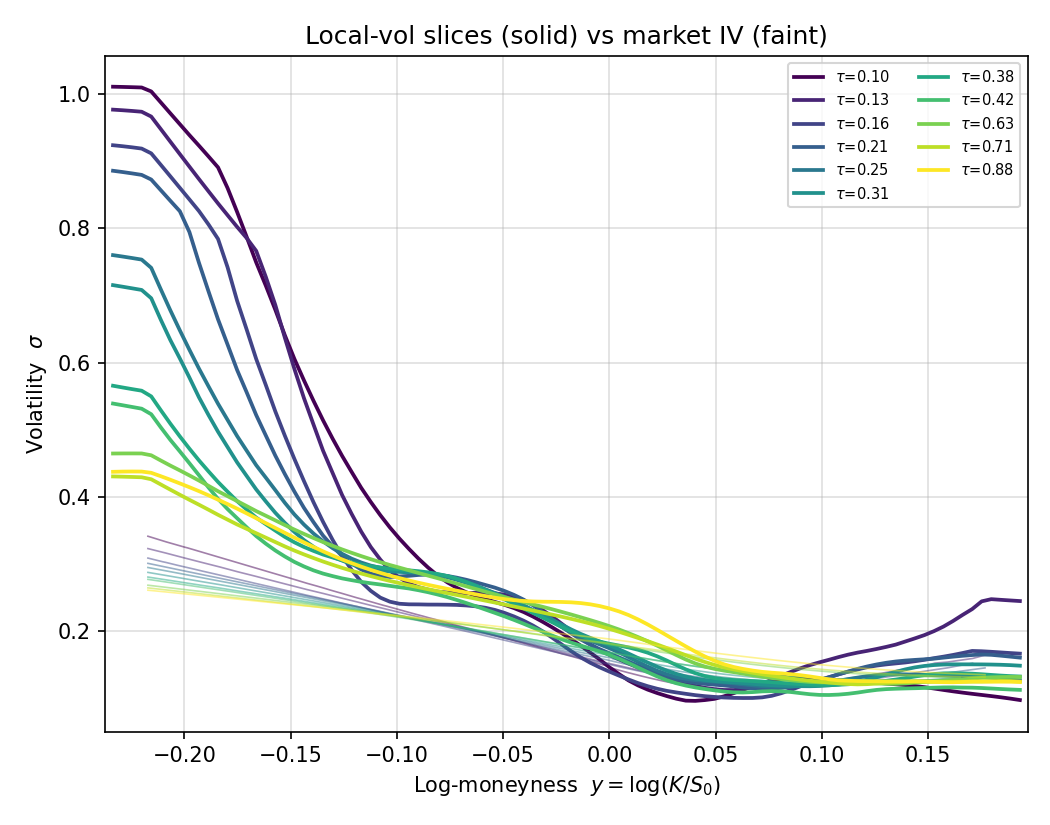
\includegraphics[width=\linewidth]{egger_example4_surface_slices}
    \caption{\scriptsize Local (solid) vs.\ implied (faint) volatility.}
    \end{subfigure}
\end{figure}
\begin{scriptsize}
Pronounced negative skew: $\lvol \approx 0.15$ ATM at the short end to $0.23$ at the long end,
up to $0.95$ on the short downside.
Median reprice error $0.13\%$, below $1\%$ on liquid strikes at every maturity
(the naive prior $\tfrac12\ivol^2$ gives $0.20\%$ and maxima above $2\%$).
\end{scriptsize}
\end{frame}

\begin{frame}
\frametitle{Market surface. Free of arbitrage by construction}
\begin{scriptsize}
\begin{itemize}
\item The optimizer keeps $a \geq 10^{-8}$ and the prices solve the Dupire equation with that coefficient,
so they are the prices of a genuine diffusion: the conditions of the no-arbitrage slide cannot fail.
\item The implied volatility interpolation route carries no such guarantee.
\end{itemize}
\end{scriptsize}
\begin{figure}[htb!]
    \centering
    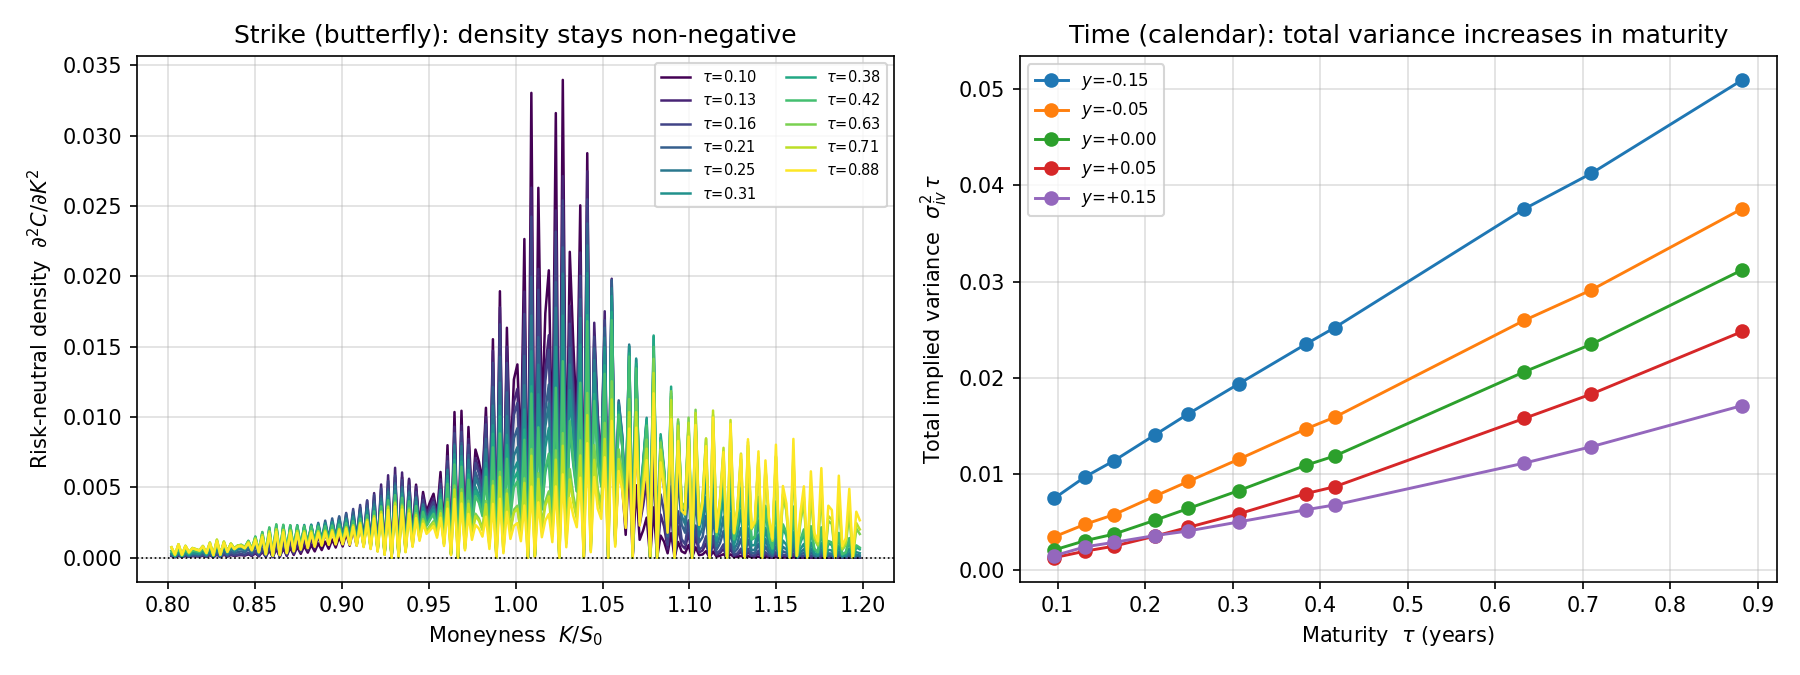
\includegraphics[width=\linewidth]{egger_example7_arbitrage}
    \caption{\scriptsize Left: risk-neutral density $\partial^2_{KK}\mathcal{C} \geq 0$ per maturity (no butterfly arbitrage).
    Right: total implied variance $\ivol^2\tau$ increasing in maturity (no calendar arbitrage).}
\end{figure}
\end{frame}

\begin{frame}
\frametitle{Market surface. The rule of two}
\begin{scriptsize}
Near the money $\partial_y \lvol|_{y=0} = 2\,\partial_y \ivol|_{y=0}$.
Quadratic fits on $|y| \le 0.05$ of the market smile and of the calibrated slices:
\end{scriptsize}
\begin{figure}[htb!]
    \centering
    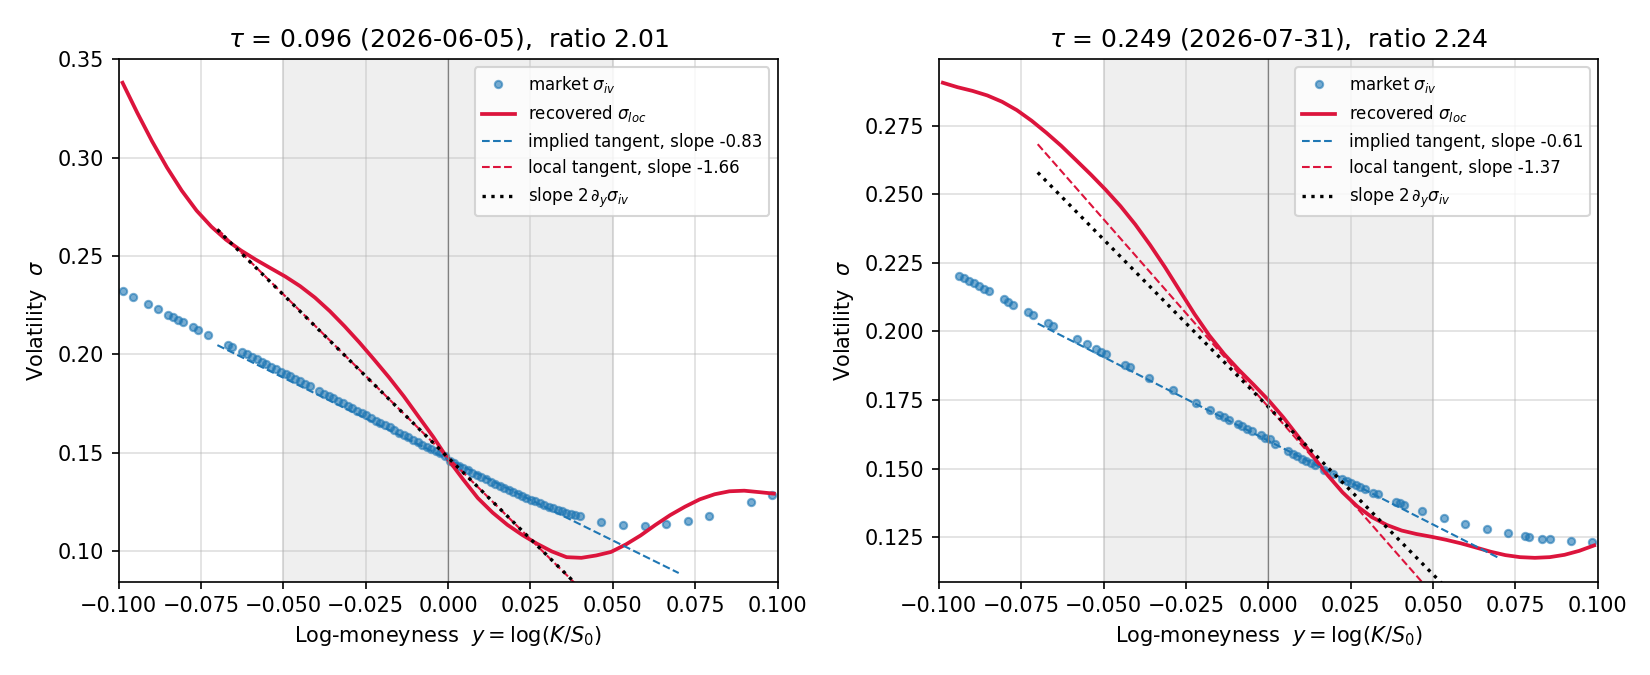
\includegraphics[width=0.8\linewidth]{egger_example5_skew}
\end{figure}
\begin{center}
\begin{tiny}
\setlength{\tabcolsep}{4pt}
\begin{tabular}{c c c c c c c c c c c c}
\toprule
$\tau$ & 0.096 & 0.132 & 0.164 & 0.211 & 0.249 & 0.307 & 0.384 & 0.416 & 0.633 & 0.710 & 0.882 \\
\midrule
ratio & 2.01 & 2.17 & 2.02 & 2.36 & 2.24 & 2.32 & 2.19 & 2.24 & 2.47 & 2.17 & 2.38 \\
\bottomrule
\end{tabular}
\end{tiny}
\end{center}
\begin{scriptsize}
The ratio averages $2.16$ below three months and stays in $[2.0, 2.5]$: the theory is confirmed empirically.
\end{scriptsize}
\end{frame}

\begin{frame}
\frametitle{Market surface. Out of sample pricing}
\begin{scriptsize}
Remove the December 2026 expiration ($\tau = 0.63$) and price it out of sample:
\begin{itemize}
\item \textbf{Local volatility}: calibrate on the other ten maturities, the Dupire equation propagates across the gap.
\item \textbf{Implied volatility}: interpolate the total variance $\ivol^2\tau$ linearly between $\tau = 0.42$ and $0.71$.
\end{itemize}
\end{scriptsize}
\begin{figure}[htb!]
    \centering
    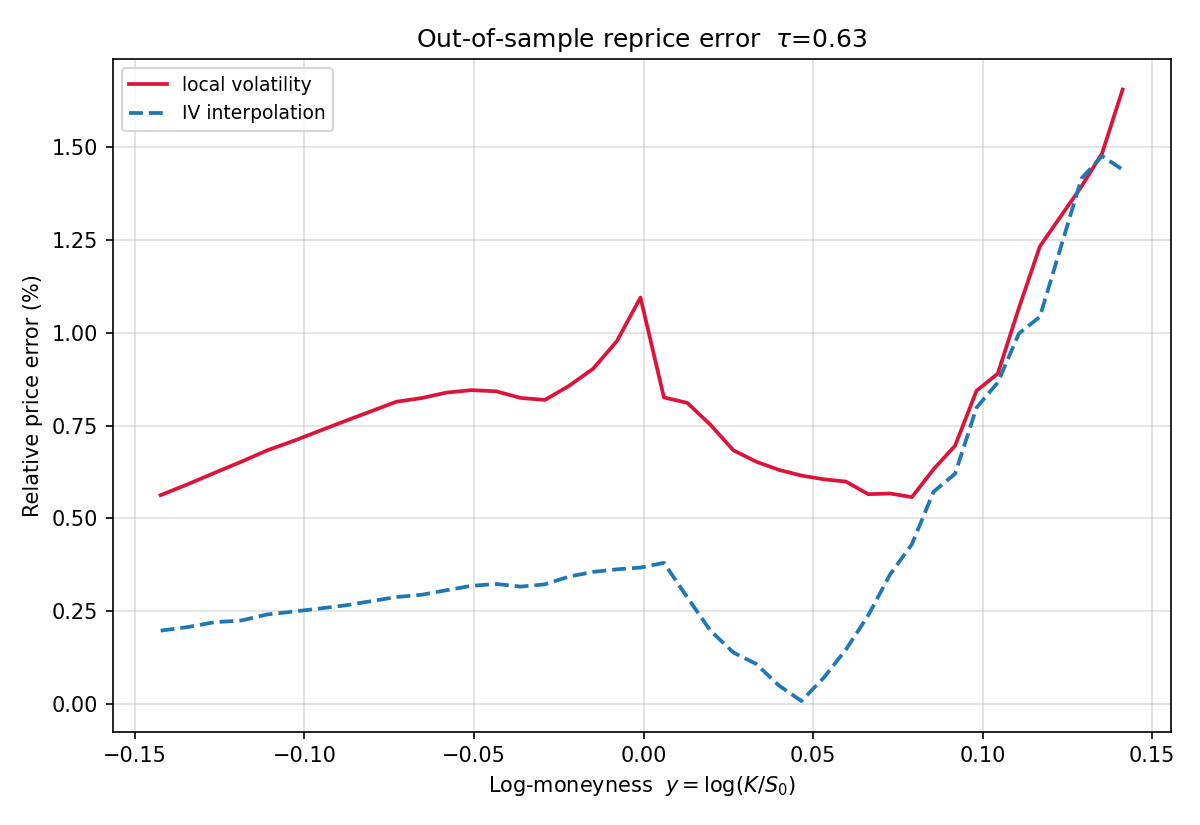
\includegraphics[width=0.55\linewidth]{egger_example6_holdout}
\end{figure}
\begin{scriptsize}
Neither is off by more than $2\%$ on $|y| \le 0.15$.
Median error: $0.75\%$ local volatility, $0.29\%$ interpolation.
the interpolation is built to reproduce the smile, while the local volatility error accumulates through the PDE.
Yet only the local volatility surface is guaranteed to be arbitrage-free.
\end{scriptsize}
\end{frame}

% ----------------------------------
%   Conclusions and references
% ----------------------------------

\begin{frame}
\frametitle{Conclusions}
\begin{scriptsize}
\begin{itemize}
\item We built the pricing theory from stochastic calculus, through Black-Scholes and arbitrage theory,
up to the Dupire forward equation and its no-arbitrage conditions.
\item Calibration of local volatility is an ill-posed inverse problem,
and Tikhonov regularization with an adjoint gradient solves it at the cost of two PDE solves per iteration.
\item We reproduced the examples of Egger and Engl:
the data determine the volatility near the money, the prior determines the wings.
\item We extended the framework to a time dependent coefficient and calibrated a full SPY surface,
arbitrage-free by construction, with sub-percent reprice errors.
\item The rule of two is confirmed empirically on the calibrated surface,
and the model reprices a held-out maturity within $2\%$.
\end{itemize}
\medskip

\textbf{Further work}
\begin{itemize}
\item Convergence results for the time dependent extension.
\item Inverse problem formulations for random data, closer to market conditions.
\end{itemize}
\end{scriptsize}
\end{frame}

\frame
{\frametitle
{References}
\scriptsize{
\begin{enumerate}
\item Bergomi, L. (2015). \emph{Stochastic Volatility Modeling}. CRC Press.
\item Berestycki, H., Busca, J., Florent, I. (2002). \emph{Asymptotics and calibration of local volatility models}. Quantitative Finance.
\item Bj\"ork, T. (2009). \emph{Arbitrage Theory in Continuous Time}. Oxford University Press.
\item Black, F., Scholes, M. (1973). \emph{The Pricing of Options and Corporate Liabilities}. Journal of Political Economy.
\item Breeden, D. T., Litzenberger, R. H. (1978). \emph{Prices of State-Contingent Claims Implicit in Option Prices}. Journal of Business.
\item Derman, E., Miller, M. B., Park, D. (2016). \emph{The Volatility Smile}. Wiley.
\item Dupire, B. (1994). \emph{Pricing with a Smile}. Risk.
\item Egger, H., Engl, H. W. (2005). \emph{Tikhonov regularization applied to the inverse problem of option pricing: convergence analysis and rates}. Inverse Problems.
\item Engl, H. W., Hanke, M., Neubauer, A. (1996). \emph{Regularization of Inverse Problems}. Kluwer.
\item Merton, R. C. (1973). \emph{Theory of Rational Option Pricing}. Bell Journal of Economics and Management Science.
\item Steele, J. M. (2010). \emph{Stochastic Calculus and Financial Applications}. Springer.
\end{enumerate}
}
}

\begin{frame}
\begin{center}
\Large Thank you
\end{center}
\end{frame}


\end{document}
